\documentclass[twocolumn]{article}
\usepackage[a4paper, top=1in, bottom=1in, left=2cm, right=2cm]{geometry}
\usepackage[singlespacing]{setspace}
\usepackage{amsmath}
\usepackage{amssymb}
\usepackage{graphicx}
\usepackage{hyperref}
\title{From Everyday to Extraordinary:\\ The Astroid Revealed in a Glass of Water}
\author{M. Ryu \\ {\href{mailto:mingshey@hafs.hs.kr}{mingshey@hafs.hs.kr}}}
\begin{document}
\maketitle
%
\newcommand{\romana}{{a}}
\newcommand{\romanb}{{b}}
\newcommand{\romanA}{{A}}
\newcommand{\romanB}{{B}}
\newcommand{\greeka}{{\alpha}}
\newcommand{\greekb}{{\beta}}
\newcommand{\Aprime}{{A^{\prime}}}
\newcommand{\Bprime}{{B^{\prime}}}
%
\section{Introduction}

A pencil partially immersed in water, appearing bent, is a common phenomenon encountered when first learning about refraction (Figure \ref{fig:pencil}). However, the apparent position of the pencil tip varies depending on the viewing angle, a phenomenon that warrants further investigation.

\begin{figure}[ht]
	\centering
	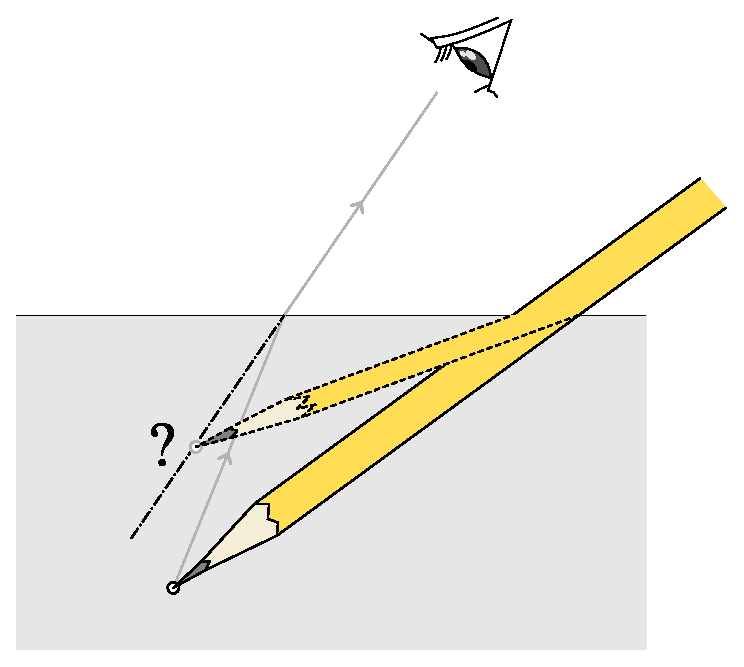
\includegraphics[width=2in]{g164.eps}
	\caption{A pencil appearing bent in water}
	\label{fig:pencil}
\end{figure}

Typically, introductory physics courses cover the apparent depth when viewed vertically. However, a detailed analysis of how the apparent position changes when viewed obliquely is often omitted. Even advanced optics textbooks tend to gloss over this phenomenon, focusing instead on more fundamental topics such as lenses and mirrors.

This is perhaps because a rigorous analysis of this phenomenon requires a level of mathematical sophistication that may be beyond the scope of introductory courses, and its practical applications may be considered less significant compared to the workings of optical instruments. 

Nevertheless, this seemingly simple yet intriguing phenomenon continues to spark curiosity. The author believes that many others have pondered this question as well. This paper aims to provide an answer.


\section{Quick Answer}

For those who are curious but short on time, here's the bottom line: When viewing a point object submerged in water from above, the apparent position of the image varies depending on the point of view. As the viewing point moves, the locus of the observed image on the normal plane forms a type of caustic\footnote{In this case you could call it a \emph{virtual caustic}, since it's the locus of virtual images}, which in this case is a curve known as a \emph{squashed astroid}.

\begin{figure}[h]
	\centering
	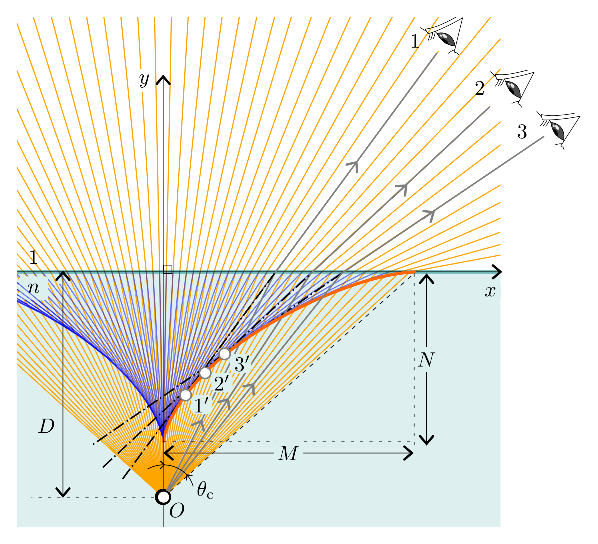
\includegraphics[width=3in]{g409.eps} \hfill\null
	\caption{Locus of the image point as the viewing point moves}
	\label{fig:caustic}
\end{figure}

Considering the normal plane containing both the object and the viewer, with the intersection of the plane and the water surface as the $x$-axis and the normal passing through the object as the $y$-axis, as shown in Figure \ref{fig:caustic}, the locus of the image can be described by the following equation:

$$ \left| \dfrac{x}{M} \right| ^ {2/3} + \left| \dfrac{y}{N} \right| ^ {2/3} = 1,$$
where $M = D/\sqrt{n^2 - 1}$ is the maximum incident distance determined by the critical angle of total internal reflection ($\theta_{\mathrm{c}}$), $N = D/n$ is the apparent depth when viewed directly from above, $D$ is the actual depth of the object, and $n$ is the refractive index of water relative to air.

\section{Derivation of the Equation}

Consider a point object O submerged at a depth D below the interface between air and water with refractive indices $n_1$ and $n_2$, respectively. A ray of light emanating from the object intersects the interface at point A, located a distance $\alpha$ from the y-axis. The ray makes an angle $\theta_2$ with the normal at point A and is refracted into the air at an angle $\theta_1$ with respect to the same normal.

As the angle of incidence $\theta_2$ varies, the extension of the refracted rays envelop a curve, known as the caustic. The image of the object is formed at the point of tangency between the refracted ray and the caustic.

As $\theta_2$ varies, the varying refracted rays glide along a smooth curve. This kind of curve is generally called an envelope, and in optics such overlapping envelope of rays is called a caustic.
The image point $\mathrm{C}$ is located at the tangency point of the line segment $\overline{\mathrm{AB}}$ and this caustic, as it represents the local point of divergence for a neighboring pencil of rays.

\begin{figure}[h]
	\centering
	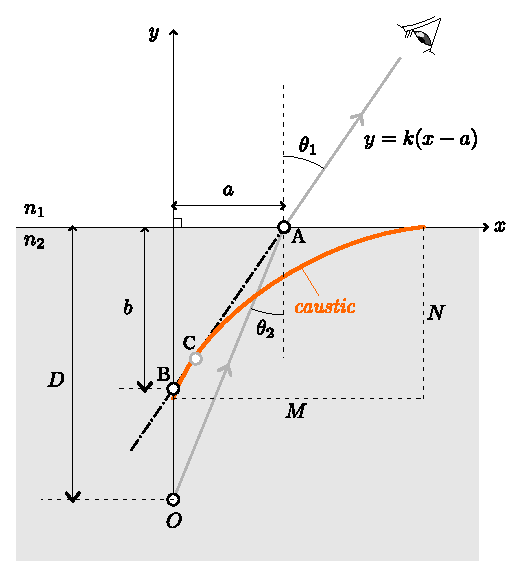
\includegraphics[width=3in]{g237.eps}
	\caption{Geometry of refraction at the air-water interface and the caustic.}
	\label{fig:geometry}
\end{figure}

Snell's law says that
$$ \sin\theta_1 = \frac{n_2}{n_1} \sin\theta_2 = n\sin\theta_2.$$

The extension of the refracted ray can be expressed by the equation
$$y=k(x-\alpha).$$
Here, 
$$k=\dfrac{1}{\tan\theta_1}=\dfrac{\cos\theta_1}{\sin\theta_1},$$
and considering Snell's law,
$$k=\dfrac{\sqrt{1-n^2\sin^2\theta_2}}{n\sin\theta_2}.$$
This line intersects the $y$-axis at point B($y=\beta$), thus
$$\beta = -k\alpha.$$
From the geometry, we obtain 
$$\alpha = D\tan\theta_2 = \dfrac{D\sin\theta_2}{\cos\theta_2}.$$
Therefore,
$$\begin{aligned}
	\beta &= -k\alpha \\
	&= -\dfrac{D\sin\theta_2}{\cos\theta_2}
	\dfrac{\sqrt{1-n^2\sin^2\theta_2}}{n\sin\theta_2}\\
	&=-\dfrac{D\sqrt{1-n^2\sin^2\theta_2}}{n\cos\theta_2}.
\end{aligned}$$

Introducing dimensionless parameters $\greeka=\romana/M$ and $\greekb=\romanb/N$, we have
$$ \begin{aligned}
	\greeka^2 + \greekb^2 &= \dfrac{\romana^2}{M^2}+\dfrac{\romanb^2}{N^2}\\
	&=\dfrac{n^2-1}{D^2}\dfrac{D^2\sin^2\theta_2}{\cos^2\theta_2}%
	+\dfrac{n^2}{D^2}\dfrac{D^2(1-n^2\sin^2\theta_2)}{n^2\cos^2\theta_2}\\
	&=\dfrac{\left(n^2-1\right)\sin^2\theta_2 + 1-n^2\sin^2\theta_2}
	{\cos^2\theta_2}\\
	&=\dfrac{1-\sin^2\theta_2}{\cos^2\theta_2}\\
	&= 1.
\end{aligned}$$
Now, introducing dimensionless coordinates $\xi=x/M$ and $\eta=y/N$, as the point of observation moves in the $xy$-plane, the corresponding points $\mathrm{\Aprime}(\alpha, 0)$ and $\mathrm{\Bprime}(0, \beta)$ in the $\xi\eta$-plane also move, maintaining a constant distance of 1. 

When a family of line segments $\overline{\mathrm{\Aprime\Bprime}}$ is overlaid, where each segment is defined by the parameter $\alpha$, the envelope formed is a well-known curve called an \emph{astroid}\footnote{not to be confused with an asteroid}, described by the equation:

$$ \left| \xi \right|^{2/3} + \left| \eta \right|^{2/3} = 1. $$

\begin{figure}[h]
	\centering
	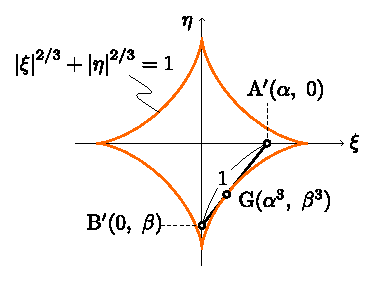
\includegraphics{g107.eps}	
	\caption{Projection of the caustic onto the $\xi\eta$ plane, revealing an astroid shape.}
	\label{fig:astroid}
\end{figure}

The point of tangency between the line segment $\overline{\mathrm{\Aprime\Bprime}}$ and the astroid is denoted by $\mathrm{G}(\greeka^3, \greekb^3)$, and this point corresponds to the image point C. 

Therefore, the coordinates of the image point $(x_{\mathrm{C}}^{}, y_{\mathrm{C}}^{})$ can be obtained from the following relations:
$$ \left\{ 
\begin{aligned}
	\xi_{\mathrm{G}}^{} &= \dfrac{x_{\mathrm{C}}^{}}{M} = \greeka^3 = \dfrac{\romana^3}{M^3},\\
	\eta_{\mathrm{G}}^{} &= \dfrac{y_{\mathrm{C}}^{}}{N} = \greekb^3 = \dfrac{\romanb^3}{N^3}.
\end{aligned}
\right.$$
That is,
$$ \left\{ 
\begin{aligned}
	x_{\mathrm{C}}^{} &= \dfrac{\romana^3}{M^2},\\
	y_{\mathrm{C}}^{} &= \dfrac{\romanb^3}{N^2}=-\dfrac{k^3\romana^3}{N^2}.
\end{aligned}
\right.$$

Using 
$$\sin\theta_2 = \dfrac{\romana}{\sqrt{D^2+\romana^2}},$$
we obtain
$$k = \dfrac{\sqrt{D^2-(n^2-1)\romana^2}}{n\romana},$$
and the position of the image can be expressed as parametric functions of $\romana$:
$$ \left\{ 
\begin{aligned}
	x_{\mathrm{C}}^{} &= (n^2-1)\dfrac{\romana^3}{D^2},\\
	y_{\mathrm{C}}^{} &= -\dfrac{n^2}{D^2}\dfrac{\romana^3}
	{n^3\romana^3}\left\{ D^2-(n^2-1)\romana^2 \right\}^{3/2}\\
	&=-\dfrac{D}{n}\left\{ 1-(n^2-1)\dfrac{\romana^2}{D^2} \right\}^{3/2}.
\end{aligned}
\right.$$

\section{When the viewpoint is submerged in water}

Consider an object located at a height D above the boundary between air and water. When the observer is submerged in water, the relative refractive index is less than 1, i.e., $1/n < 1$. Through similar reasoning, we can derive the following equation for the caustic:
$$ \left| \xi \right|^{2/3} - \left| \eta \right|^{2/3} = -1, $$
where $\xi = \dfrac{x}{W} $, $\eta = \dfrac{y}{Z}$, $W = \dfrac{nD}{\sqrt{n^2-1}}$, and $Z = nD$. This curve exhibits asymptotes with slopes of $\pm Z/W = \pm \sqrt{n^2-1}$. 

Consequently, the view of the sky observed from underwater is compressed into a circular region (or more accurately, a cone) bounded by the critical angle of total internal reflection, commonly known as Snell's window. This circular, wide-angle view, as perceived by an underwater observer, resembles the field of view of a fisheye lens.

A more general form of this curve is given by 
$$ \left| \xi \right|^{r} - \left| \eta \right|^{r} = \pm1, $$
which is referred to as a \emph{super hyperbola} in \href{http://dynamicmathematicslearning.com/super-ellipse.html}{DML}\footnote{\ttfamily{dynamicmathematicslearning.com/super-ellipse.html}}. In the \href{https://old.nationalcurvebank.org/superconicncb/superconicncb.htm}{National Curve Bank}\footnote{\ttfamily{old.nationalcurvebank.org/superconicncb/\\superconicncb.htm}}, these curves, along with the \emph{super-ellipses} defined by
$$ \left| \xi \right|^{r} + \left| \eta \right|^{r} = 1, $$
are collectively termed \emph{superconics}. (An astroid belongs to the super-ellipses.) 

The specific case where 
$$ \left| \xi \right|^{2/3} - \left| \eta \right|^{2/3} = \pm1, $$
has physical significance as the caustic of rays emanating from a point light source above water and refracted into water. Given its relationship to the astroid, which is analogous to the relationship between a hyperbola and an ellipse, we propose the term \emph{hyperastroid} for this curve.

\begin{figure}[h]
	\centering
	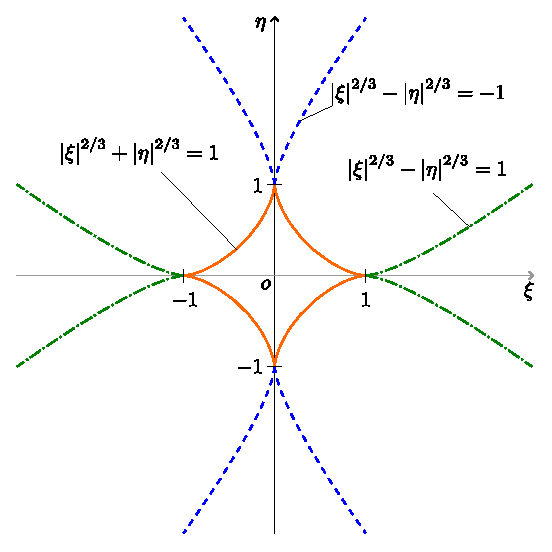
\includegraphics[width=3in]{g254.eps}
	\caption{Astroid and `\emph{hyperastroids}'}
	\label{fig:hyperastroid}
\end{figure}

\section{Finding the Image Location}

The closed-form caustic curve can be utilized to determine the location of an image given the position of an object and the viewpoint.

\begin{figure}[h]
	\centering
	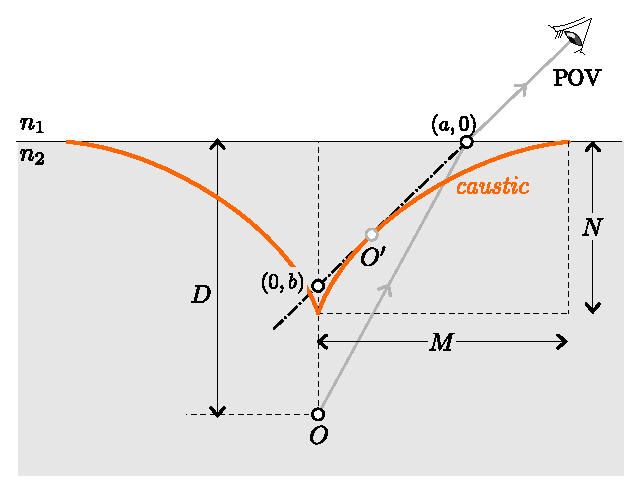
\includegraphics[width=3in]{g394.eps}
	\caption{Determining the image location using the caustic curve}
	\label{fig:image_caustic}
\end{figure}

A tangent is drawn from the viewpoint to the caustic curve. The point of tangency represents the location of the image, and the intersection of the tangent with the water surface corresponds to the point where the light ray from the object strikes the surface.

For a continuous object submerged in water, we can find the image of each point on the object by repeating this process. The locus of these image points will form the image of the entire object.

\begin{figure}[h]
	\centering
	\includegraphics*[width=3in]{g240.eps}
	\caption{Image of a continuous object}
	\label{fig:extended_image}
\end{figure}

However, determining the tangent to the caustic analytically can be challenging. In practice, numerical methods are often used to approximate the tangent point.

Alternatively, we can numerically solve for the path of a light ray connecting the object and the viewpoint using Fermat's principle. By finding the intersection of this ray with the water surface, we can then use the equation of the astroid to determine the corresponding image point. A Python implementation of this method can be found at  \href{https://github.com/mingshey/python\_projects/blob/main/Refraction\_Image\_en.ipynb}{\sffamily{github}}\footnote{\ttfamily{https://github.com/mingshey/python\_projects/\\blob/main/Refraction\_Image\_en.ipynb}}.

\appendix
\newcommand{\pd}[2]{{\frac{\partial #1}{\partial #2}}}
\newcommand{\ilpd}[2]{{{\partial #1}/{\partial #2}}}
\section*{Appendix: The Astroid as an Envelope}

Consider a Cartesian coordinate system with a point $(a, 0)$ on the x-axis and a point $(0, b)$ on the y-axis, moving such that the distance between them remains constant at $c$. Thus, $a^2+b^2=c^2$. The equation of the line connecting these two points at any given time can be expressed as:

$$y=-\dfrac{b}{a}(x-a)$$

By substituting $b=\pm \sqrt{c^2-a^2}$, we obtain

$$y(x, a) = \mp \dfrac{\sqrt{c^2-a^2}}{a}(x-a)$$

As the value of $a$ varies, the line connecting the two points also changes. The envelope of this family of lines is defined as the locus of points that are stationary as $a$ varies infinitesimally, that is, the points where $\ilpd{y}{a} = 0$. To find these points, we differentiate $y$ with respect to $a$:

$$ \begin{aligned}
	\pd{y}{a} &= \pm\left[\left( \dfrac{1}{\sqrt{c^2-a^2}}+\dfrac{\sqrt{c^2-a^2}}{a^2}\right) (x-a) + \dfrac{\sqrt{c^2-a^2}}{a} \right]\\
	&= \pm \dfrac{(a^2+c^2-a^2)(x-a)+a(c^2-a^2)}{a^2\sqrt{c^2-a^2}}\\
	&= \pm \dfrac{c^2 x - a^3}{a^2 \sqrt{c^2 - a^2}}\\
	&= 0.
\end{aligned}
$$

Therefore, the $x$-coordinate of the stationary point is $x = a^3/c^2$, and substituting this into the equation for $y$, we find the $y$-coordinate to be

$$ \begin{aligned}
	y(x, a) &= \mp \dfrac{\sqrt{c^2-a^2}}{a}\left(\dfrac{a^3}{c^2}-a\right)\\
	& = \pm \dfrac{\left( c^2- a^2 \right)^{3/2}}{c^2}\\
	& = \dfrac{b^3}{c^2}
\end{aligned}
$$

Thus, the coordinates $(x, y)$ of the stationary points satisfy the equation
$$ \left|\dfrac{x}{c}\right|^{2/3} + \left|\dfrac{y}{c}\right|^{2/3} = 1. $$
$\blacksquare$

\section*{Acknowledgments}
The author would like to thank Google's Gemini language model for its assistance with the translation of this document from Korean.

\end{document}

